\section{Results}

\subsection*{Phase 1: LLM Labeling}

\begin{table}[!ht]
\centering
\caption{\textbf{Labeler Statistics}}
\label{tab:labeler-results}
\begin{tabular}{lllccc}
\toprule
 &  &  &  \textbf{LPP} & \textbf{Cost} & \textbf{M.-F1} \\
\textbf{Model} & \textbf{Context} & \textbf{Shot} & ($\mu\pm\sigma$) & (\$) & (\%) \\
\midrule
\multirow[c]{6}{*}{
    \rotatebox[origin=c]{90}{GPT-3.5}
    } & \multirow[c]{2}{*}{\texttt{context1}} & 0-shot & 0.39 ± 0.61 & \textbf{0.36} & 15.96 \\
 &  & 1-shot & 0.91 ± 0.95 & 0.48 & 23.26 \\
 & \multirow[c]{2}{*}{\texttt{context2}} & 0-shot & 1.39 ± 0.98 & 0.42 & 37.59 \\
 &  & 1-shot & 1.68 ± 1.15 & 0.63 & 38.69 \\
 & \multirow[c]{2}{*}{\texttt{context3}} & 0-shot & 1.57 ± 1.08 & 0.57 & 37.24 \\
 &  & 1-shot & 1.85 ± 1.24 & 0.80 & 37.70 \\
\midrule
\multirow[c]{6}{*}{
    \rotatebox[origin=c]{90}{GPT-4}
    } & \multirow[c]{2}{*}{\texttt{context1}} & 0-shot & 1.50 ± 0.93 & 4.68 & 35.55 \\
 &  & 1-shot & 1.83 ± 1.36 & 5.75 & 36.10 \\
 & \multirow[c]{2}{*}{\texttt{context2}} & 0-shot & 2.16 ± 1.03 & 5.26 & 45.39 \\
 &  & 1-shot & 2.49 ± 1.28 & 7.25 & 45.93 \\
 & \multirow[c]{2}{*}{\texttt{context3}} & 0-shot & 2.30 ± 1.11 & 6.68 & 44.10 \\
 &  & 1-shot & 2.80 ± 1.30 & 8.99 & \textbf{46.12} \\
\bottomrule
\end{tabular}
\end{table}


Table~\ref{tab:labeler-results} presents important statistics of the re-labelling of the original crowdsourced corpus of websites using the LLM labelers introduced in Section \ref{sec:methodology}.

% General Results: Consistency, Cost, Quality
\textbf{Results.} Our findings demonstrate that LLM labelers can provide \textit{consistent}, \textit{cost-effective}, and \textit{high-quality} annotations for the complex task of multi-lingual, multi-label website topic classification. 

% Consistency
Remarkably, not a single incorrect output was produced, underscoring the reliability and consistency of LLM-generated annotations.

% Cost
In terms of cost, the labeling of the original crowdsourced corpus cost approximately \$130 per 1000 pages. Our approach, utilising GPT-3.5 and GPT-4 labelers, drastically reduces this cost to an average of \$0.54 and \$6.44, respectively, achieving a reduction by factors of 240x and 20x.

% Calculations
% Human annotator cost: 327 USD
% Pages annotated: 840 * 3 = 2520
% Cost per 1k page: 1000 * 327 / 2520 = 130$

% GPT-3.5 labler cost/1k pages:
% (0.36 + 0.48 + 0.42 + 0.63 + 0.57 + 0.80) / 6 = 0.54

% GPT-4 labler cost/1k pages:
% (4.68 + 5.75 + 5.26 + 7.25 + 6.68 + 8.99) / 6 = 6.44

% Cost reductions:
% GPT-3.5: 130 / 0.54 = 240x
% GPT-4: 130 / 6.44 = 20x

% Performance
Performance-wise, the best-performing labeler, GPT-4 with \texttt{context3} and \texttt{1-shot} achieves a macro F1 score of 46\% score, outperforming the baseline of the pre-trained model. The improvements suggest that we can expect to improve the performance of the pre-trained model by fine-tuning it with the LLM labels if we can distil the knowledge from the LLMs into the pre-trained model - the goal of the second phase of our study.

% GPT labeler parameter grid
\textbf{Labeler Parameter Grid.} Figure~\ref{fig:labelers-grid} visualises the effect of the labeler parameters on the macro F1 score. As expected, we find that the quality of the labels increases with the amount of context provided and the quality of the model used. Interestingly, the added feature in the context3 (links and text) do not increase the annotation quality for the GPT-3.5, but do for the GPT-4. We hypothesise that this is due to the fact that the smaller model can get confused with the the additional features that are very long compared to the prompt, while the larger model is superior in handling the additional features.

\begin{figure}[!h]
    \centering
    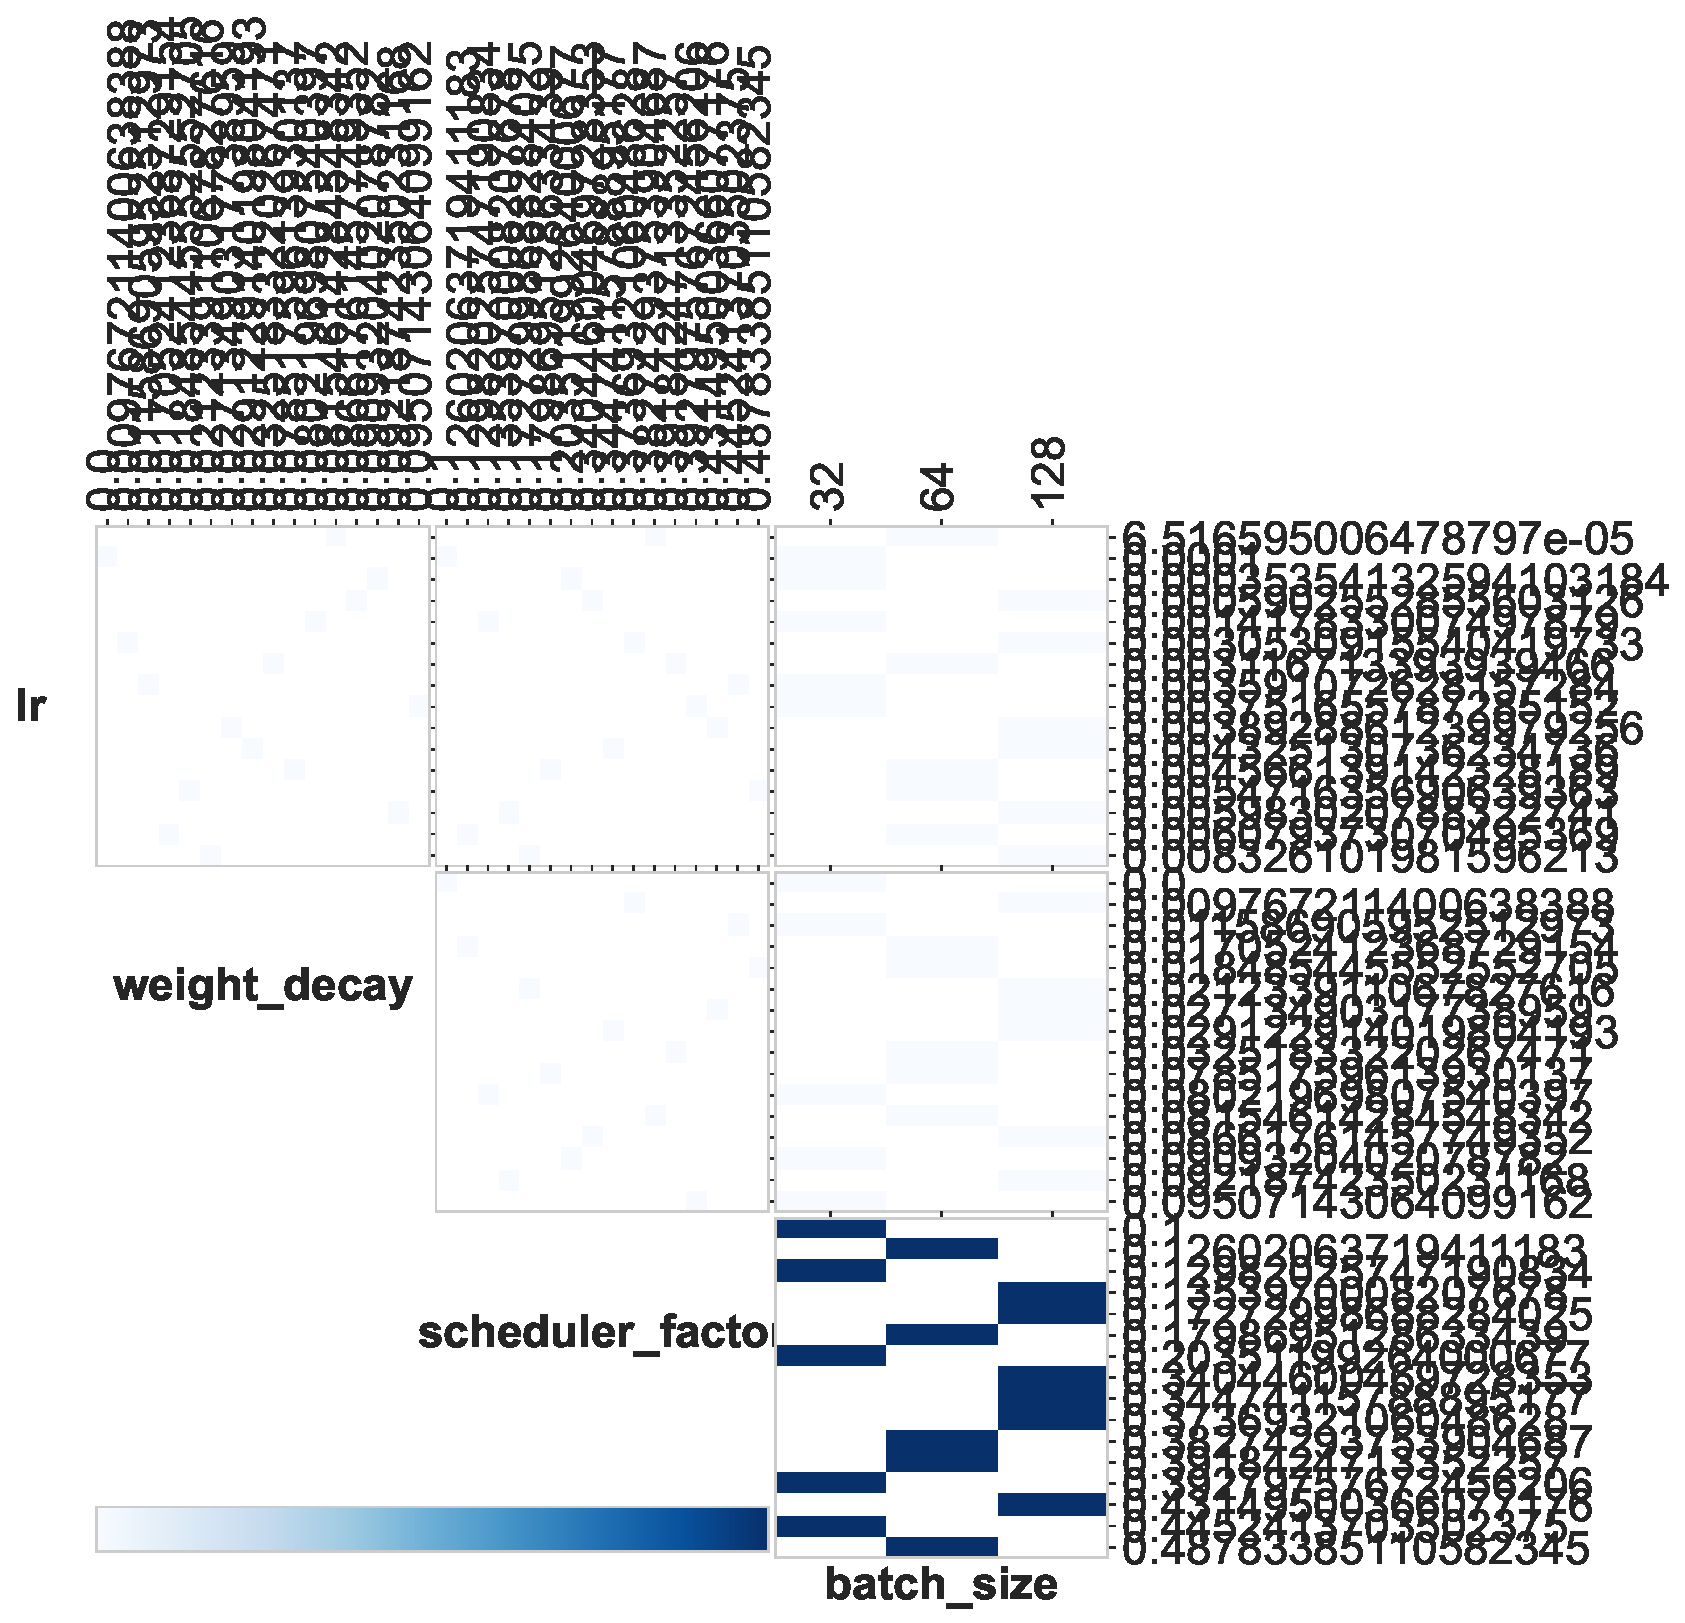
\includegraphics[width=.8\columnwidth]{figures/labeler-grid.pdf}
    \caption{\textbf{Labeler Parameter Grid.} The Figure displays the mean macro F1 score for all unique parameter combinations of the LLM labelers.}
    \label{fig:labelers-grid}
\end{figure}

% Cost-quality trade-off
\textbf{Cost-Quality Trade-Off.} 
Out analysis reveals a positve trend between label quality and cost, attributable to the use of longer prompts or more sophisticated models. The optimal compromise is achieved with a GPT-3.5 annotator utilizing \texttt{context2} and a few-shot example. This configuration ensures a robust label quality at 39\% (only a 15\% decrease) while cutting the cost per 1000 pages from \$7.25 to \$0.63 (a 91\% decrease). This GPT-3.5 annotator was used to label the texttt{curlie-gpt3.5-10k} dataset, which we use in the second phase of our study.

% Curlie-10k dataset
The average number of topics assigned to a page is \textbf{1.6}, which is higher than the average of \textbf{1.07} for the original Curlie dataset. Figure~\ref{fig:label-distribution-comparison} shows the distribution of the labels in the re-labelled dataset compared to the original Curlie dataset. We observe that the number of labels increased for every class.

\begin{figure}[!h]
    \centering
    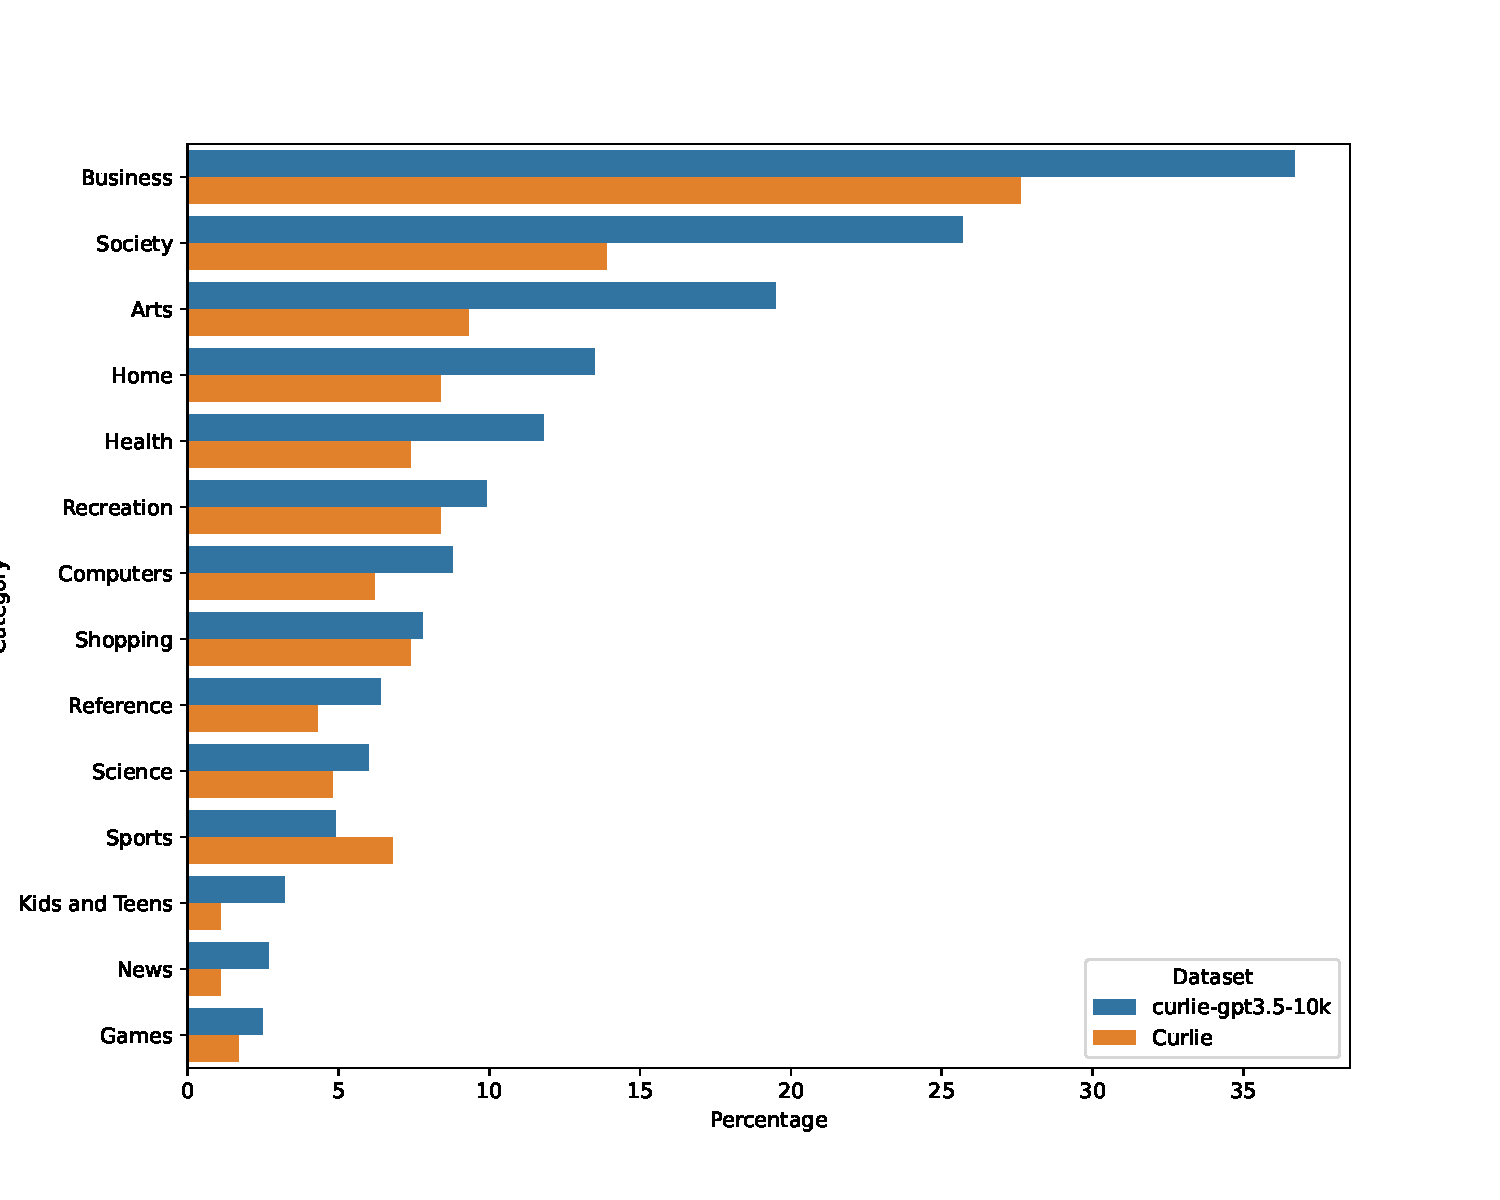
\includegraphics[width=.8\columnwidth]{figures/class_distribution_comparison.pdf}
    \caption{\textbf{Curlie-10k Label Distributino.} We show the topic distribution of the Curlie-10k dataset.}
    \label{fig:label-distribution-comparison}
\end{figure}


\subsection*{Phase 2: Knowledge Distillation}

% TODO: Would be cool to compare the labelling statistics of the exact 10k subsplit (Curlie vs. GPT) -- for now we will proxy.

The goal of the second phase of the study is to transfer the knowledge from the LLMs into the pre-trained model. 
To this end, we use the \texttt{curlie-gpt3.5-10k} dataset for fine-tuning the pre-trained model.

% Fine-tuning results
\textbf{Finetuning.} Table~\ref{tab:finetune-results} shows the results of the fine-tuning experiment. 
We observe that the fine-tuned model increases the recall significantly from 39.4\% to 47.6\%, at the cost of a minor decrease in precision from 40.9\% to 40.2\%. 
This increases the overall macro F1 score from 39.2\% to 42.6\%, which is a 9\% improvement. 
We have shown that the approach of fine-tuning the pre-trained model with the LLM labels can improve the performance on the texttt{crowdsourced} dataset that better resembles the true website topic classification.

% 0.391610 = 39.2% (Pre-trained Homepage2Vec)
% 0.426289 = 42.6% (GPT-3.5)
% Absolute Difference: 0.034679 = 3.5 percentage points
% Relative Difference: 0.086 = 8.6%

\begin{table}[!ht]
\centering
\caption{\textbf{Finetuning Results.} The table shows the precision, recall, macro F1 and and labels per page when evaluated on \texttt{crowdsourced}. We show results for the pre-trained baseline, as well as both finetuned variants.}
\label{tab:finetune-results}
\begin{tabular}{lrrrr}
\toprule
 & \textbf{Pr.} & \textbf{Re.} & \textbf{M.-F1} & \textbf{LPP} \\
 & (\%) & (\%) & (\%) & ($\mu$) \\
\midrule
Pretrained & \textbf{40.97} & 39.44 & 39.16 & 1.84 \\
GPT-3.5 & 40.19 & 47.55 & 42.63 & 1.93 \\
GPT-4 & 39.92 & \textbf{49.07} & \textbf{42.87} & \textbf{3.07} \\
\bottomrule
\end{tabular}
\end{table}


Figure~\ref{fig:finetune-results} shows the class-wise F1 score for the pre-trained model and the fine-tuned model. We observe that the fine-tuned model consistently outperforms the pre-trained model, achieving higher F1 scores in ten out of the 14 classes.

\begin{figure*}
    \centering
    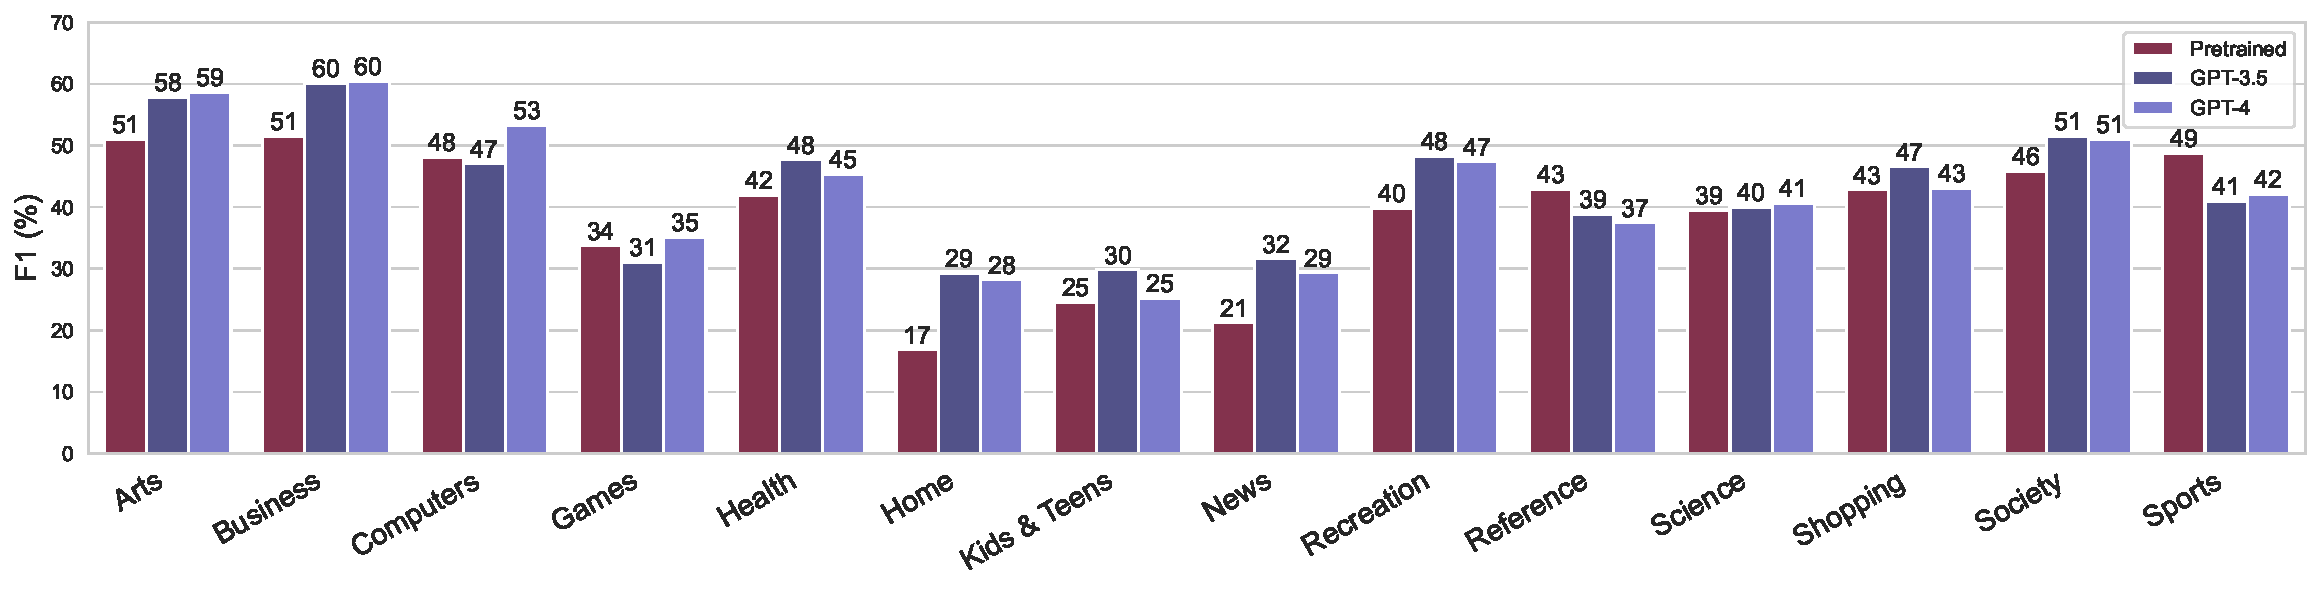
\includegraphics[width=\textwidth]{./figures/exp2-mf1.pdf}
    \caption{\textbf{Finetune Results.} Class-wise F1 score for the pre-trained model and the fine-tuned model on te original crowdsourced data.}
    \label{fig:finetune-results}
\end{figure*}
